% Created 2010-07-01 Thu 09:45
\documentclass[aps, twocolumn, groupedaddress]{revtex4}
\newcommand{\lb}{{\langle}}
\newcommand{\rb}{{\rangle}}
\usepackage{graphicx}
\usepackage{epsfig}
\usepackage{amssymb,amsmath}
\usepackage{bm}
\usepackage{pdfsync}


\usepackage{pdfsync}

\title{Draft of diameter paper}
%\author{Don Blair}
\date{01 July 2010}

\begin{document}




\section{Introduction}
\label{sec-1}
\subsection{Background to the Potts Model}
\label{sec-1.1}
\subsection{Tests of the Potts Model}
\label{sec-1.2}
\subsection{This is all we need to know}
\label{sec-1.3}
\subsection{Not much more syntax highlighting}
\label{sec-1.4}
\subsubsection{Big test}
\label{sec-1.4.1}
\subsubsection{Other test}
\label{sec-1.4.2}
\subsubsection{Finish the damn outline}
\label{sec-1.4.3}

Here is a test \cite{OsSo04}.  

$\lb a + b \rb$    
    
The Potts Model, initially introduced as a generalization of the 2-state Ising Model to $q$ possible spin states, can in fact be mapped onto the Random Cluster Model for all $q \ge 0$, with $q \to 1$ corresponding to the Percolation Model, and $q \to 2$ corresponding to the Ising Model.  The Potts Model has found application in an impressively diverse range of applications, including conformal field theory, percolation theory, knot theory, quantum groups, mathematical biology, and complex networks.    
\%more specific \ldots{}    
Although easy to formulate, the model exhibits rich phase behavior, and its study has yielded many significant insights into critical phenomena in statistical physics. 

An important \textbf{geometric} property of Potts clusters that has proved very useful in describing transport and diffusion processes in random media is the ``chemical distance'', $l$ -- the length of the ``chemical'' or shortest path between two randomly chosen sites on a cluster.  The average chemical distance on critical Potts clusters has been shown to scale as $\bar{l} \propto r^{d_{min}}$ at criticality, where $r$ is the Euclidean distance between the endpoints of the chemical path $l$. Attempts to establish a relationship between $d_{min}$ and other known critical exponents have, as yet, proved inconclusive [refs].  For the $q \to 1$ (Percolation) case, much work has already been done to determine $d_{min}$ numerically \cite{Gr83, HrSt88} and an exact solution has been found using results from conformal field theory \cite{Zi99}.
 
In this paper we generalize previous studies of $d_{min}$ for the 2D, $q=1$ Potts Model by reporting results for the $q = 2, 3$ and $4$ for both Potts Models in both 2D and 3D.  We also study the critical scaling of a related quantity: the diameter, $D$, defined as the longest of all the shortest paths between points on a cluster. (An illustration of both $D$ and $l$ on a Potts cluster is shown in Figure [A]).  We show that $D$ also exhibits scaling behavior at criticality: $\bar{D} \propto r^{D_{min}}$; and that, significantly, $d_{min} = D_{min}$ to within the error of our numerical results.  
 
We also propose a possible relationship between both $D_{min}$ \$d$_{\mathrm{min}}$\$ and the dynamical exponent, $z$.


\begin{center}
\begin{tabular}{lrr}
 Name   &  Phone  &  Age  \\
\hline
 Peter  &   1234  &   17  \\
 Anna   &   4321  &   25  \\
\end{tabular}
\end{center}
\section{Methods}
\label{sec-2}
\subsection{type 1}
\label{sec-2.1}
\subsection{type 2}
\label{sec-2.2}
\subsubsection{sub-sub}
\label{sec-2.2.1}

\begin{figure}[htp]
\centering
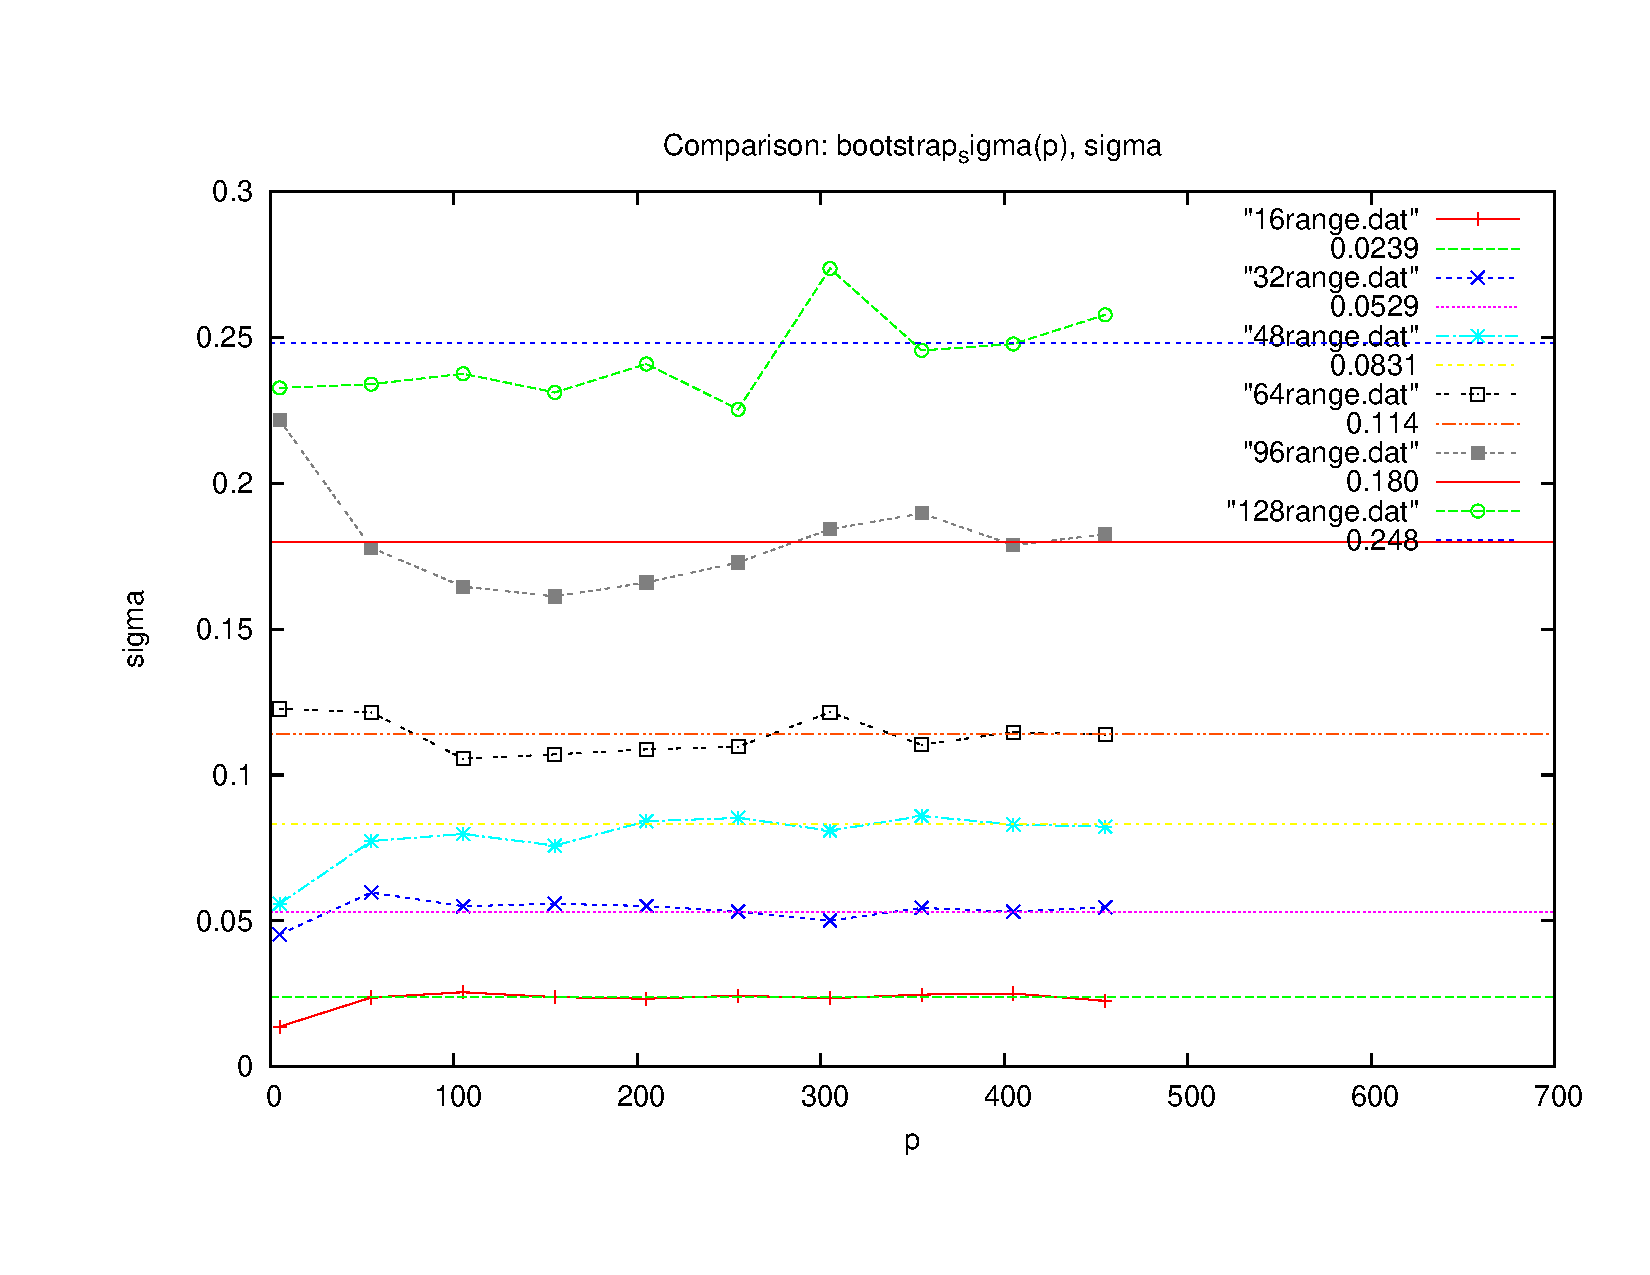
\includegraphics[width=.85\textwidth]{boot}
\caption{$d_{min}$ for D=2, q=1.}\label{fig:1}
\end{figure}
\section{Results}
\label{sec-3}
\subsection{$q=2$ and etc}
\label{sec-3.1}

This is how it'll go.

\bibliographystyle{plain}
\bibliography{/home/dwblair/Dropbox/dwbdocs/physics/writing/bibfiles/dwbreferences}

\end{document}